
\documentclass[a4paper, oneside, 11pt]{report}
\usepackage{epsfig,pifont,float,amsmath,amssymb, url, graphicx}
\newcommand{\mc}{\multicolumn{1}{c|}}
\newcommand{\mb}{\mathbf}
\newcommand{\mi}{\mathit}
\newcommand{\oa}{\overrightarrow}
\newcommand{\bs}{\boldsymbol}
\newcommand{\ra}{\rightarrow}
\newcommand{\la}{\leftarrow}
\topmargin = 0pt
\voffset = -80pt
\oddsidemargin = 15pt
\textwidth = 425pt
\textheight = 750pt

\begin{document}

\begin{titlepage}
\begin{center}
\rule{12cm}{1mm} \\
\vspace{1cm}
{\large  CMP-7009A Advanced Programming Concepts and Techniques}
\vspace{7.5cm}
\\{\Large Project Interim Report - 14 November 2018}
\vspace{1.5cm}
\\{\LARGE Evolution Sandbox}
\vspace{1.0cm}
\\{\Large Group members: \\ Benjamin Longhurst, Rupert Hammond, Ryan Phelan, Travis Payne}
\vspace{10.0cm}
\\{\large School of Computing Sciences, University of East Anglia}
\\ \rule{12cm}{0.5mm}
\\ \hspace{8.5cm} {\large Version 1.0}
\end{center}
\end{titlepage}


\setcounter{page}{1}
%\pagenumbering{roman}
%\newpage


\begin{abstract}
[TODO: write this] An abstract is a brief summary (maximum 250 words) of your entire project. It should cover your objectives, your methodology used, how you implemented the methodology for your specific results and what your final results are, your final outcome or deliverable and conclusion. You do not cover literature reviews or background in an abstract nor should you use abbreviations or acronyms. In the remainder of the report the chapter titles are suggestions and can be changed (or you can add more chapters if you wish to do so). This template is designed to help you write a clear report but you are welcome to modify it (at your peril ...). Finally, a guideline in size is approximately 3,500 words (not including abstract, captions and references) but no real limit on figures, tables, etc.
\end{abstract}

\chapter{Introduction}
An evolution simulation attempts to represent the way a set of organisms evolve within a limited ecosystem, typically a number of biological algorithms such as fitness functions and crossover are employed to dictate how this plays out. One such example of an evolution simulation is Conway's Game of Life. Created in 1970 by John Conway, the simulation takes place on an infinitely sized grid where each cell is either live or dead. It progresses according to a set of simple rules \cite{guardian}:
\begin{itemize}
	\item A live cell with less than two live neighbours becomes dead
	\item A live cell with more than four live neighbours becomes dead
	\item A dead cell with three live neighbours becomes alive
\end{itemize}

Conway's Game of Life is often praised for its ability to show how simple rules can spawn complex evolutionary patterns \cite{callahan}. This project will tackle evolution simulating by taking inspiration from Conway's Game of Life to produce a piece of software it terms an "evolution sandbox"; a simulation with emphasis on real-time manipulation and customization which will allow the user to observe the outcome of their actions on the ecosystem.

\section{MoSCoW}
In order to better understand the scope and priorities of the project, a set of analysis' were carried out with the goal of producing a MoSCoW analysis.
\smallskip 
Firstly, the basic requirement analysis was defined as follows:
\begin{itemize}\label{requirements}
	\item Organisms should act based on personal attributes, similar to the rule system in Conway's Game of Life
	\item Organism attributes should be customisable on the fly
	\item Organism attributes should mutate over generations using a crossover algorithm
	\item Organisms should utilize logical path finding when seeking
	\item The ecosystem should reach equilibrium when left to its own devices
	\item The simulation should be able to handle a large number of organisms without noticeable lag
	\item The simulation should employ realistic biological algorithms where possible
	\item The UI should be clean, simple and professional
	\item The graphics should faithfully represent the underlying simulation
\end{itemize}
\smallskip 

Next, an Object Oriented Analysis was carried out to identify the objects of the system to later be the focus of the priorities in the MoSCoW analysis:
\smallskip 
\begin{itemize}
	\item End Goal: Biological Evolution Sandbox
	\begin{itemize}
		\item What is required?
		\begin{itemize}
			\item End game, stable ecology
			\begin{itemize}
				\item Net number of organisms doesn't change
			\end{itemize}
			\item Food, vegetation, other organisms
			\item Water
			\begin{itemize}
				\item Some organisms can go in water
			\end{itemize}
			\item Weather
			\begin{itemize}
				\item Hot and cold
				\item Different types of weather
			\end{itemize}
			\item Statistics
			\item A log
			\item Disease
			\item Natural Disasters
			\item Terrain
			\item Live edit of organisms
			\item Tile-based graphics
		\end{itemize}
	\end{itemize}
\end{itemize}
\smallskip 

Finally, taking these objects and systems a MoSCoW analysis was produced:
\smallskip 
\begin{center}
	\begin{tabular}{c|p{0.8\textwidth}}\label{moscow}
		Must Have & \begin{itemize}
			\itemsep0em
			\item Organism life cycle
			\item Genetic crossover algorithm
			\item Organism attributes
			\item Live edit of organisms
			\item Simple 2D graphics
			\item Herbivores and natural food sources
		\end{itemize} \\ \hline
		Should Have & \begin{itemize}
			\itemsep0em
			\item Weather/disease system
			\item Advanced path-finding algorithm
			\item Carnivores and predator/prey organisms
			\item Terrain variation, e.g. grass, mountainous, water
			\item Ability to pause, speed up and slow down simulation
		\end{itemize} \\ \hline
		Could Have & \begin{itemize}
			\itemsep0em
			\item Natural disasters
			\item Speciation
			\item A game log with charts and text output
			\item Spritesheet animation
			\item Particle effects, e.g. weather effects, running water, blood
		\end{itemize} \\ \hline
		Won't Have & \begin{itemize}
			\itemsep0em
			\item 3D graphics
			\item Scale realism
		\end{itemize} \\
	\end{tabular}
\end{center}
\smallskip

In general, the "Must Have" objectives are those identified to be necessary to a bare minimum working product, while "Should Have" is considered a bare minimum submission. The logic being that these "Should Have" objectives could also potentially be developed further to have enough depth to utilize advanced programming techniques or have the simulation revolve around them. "Could Have" objectives are those which are considered incredibly difficult or potentially out of scope. For example, particle effects and spritesheet animation will not improve the depth of the simulation and would require effort in areas which are not programming-related. Natural disasters and speciation on the other hand would be difficult to implement while maintaining equilibrium within the ecosystem. Finally, the "Won't Have" objectives are identified to disproportionately increase the simulation's complexity when compared with the pay-off for implementing them. The implementation of this analysis is discussed in detail in Section~\ref{versioning}.

\section{Report structure}
This report will cover a brief background of evolution and the algorithms and tools which attempt to simulate it in simulators in Section~\ref{background}. Section~\ref{methodology} details the various advanced programming and project management techniques utilized in the project. The tools used and development of the product is outlined in Section~\ref{implementation}, with detail on the implementation of specific simulation components. Finally, the quality of the project will be discussed and verified through testing in Section~\ref{testing} and drawn to a conclusion in Sections \ref{discussion} and \ref{conclusion}.
 Breifly describe what you will cover in the remainder of the report, chapter by chapter.

\chapter{Background}\label{background}
[TODO: write this]
 This chapter covers a literature, resource and/or (software) product review. This means you will cite journal or conference papers outlining methodologies you may (or may not) use but which are definitely relevant to your particular problem. Resource and/or product information will typcially be substantiated through internet links. 
You may use different sections if different subareas are part of your problem statement and/or solution. 
Since this chapter covers the literature, you should also update the corresponding bib file referred to in the bottom of this document and here it is called References.bib.
You cite references like this: Taylor et al. \cite{Taylor:2007} investigated non-linear FEA on the GPU. Morton \cite{Morton:1966} developed a file sequencing method in 1966. A website on OpenCL can be found here \cite{Soos:2012}. Etc.

\chapter{Methodology}\label{methodology}

\section{Agile Methodology}\label{projectmanagement}
The project is managed according to the Agile methodology, specifically Scrum. The team meet twice per week and start with a stand-up meeting where the team give updates on the tasks they are working on and discuss solutions to problems that may have been encountered. In keeping with the Agile methodology, iterative version releases are promoted with the rule that each lab meeting must have a merged and bug-free master branch. Development is split into two to three week sprints, with the objective of producing a new product version [Section~\ref{versioning}].
GitHub is used as the centre for project management using a combination if it's project boards, where each board corresponds to one sprint and therefore one product version \ref{gitboard}, and it's issue tracking \ref{gitissue}. 

\begin{figure}[H]
	\centering
	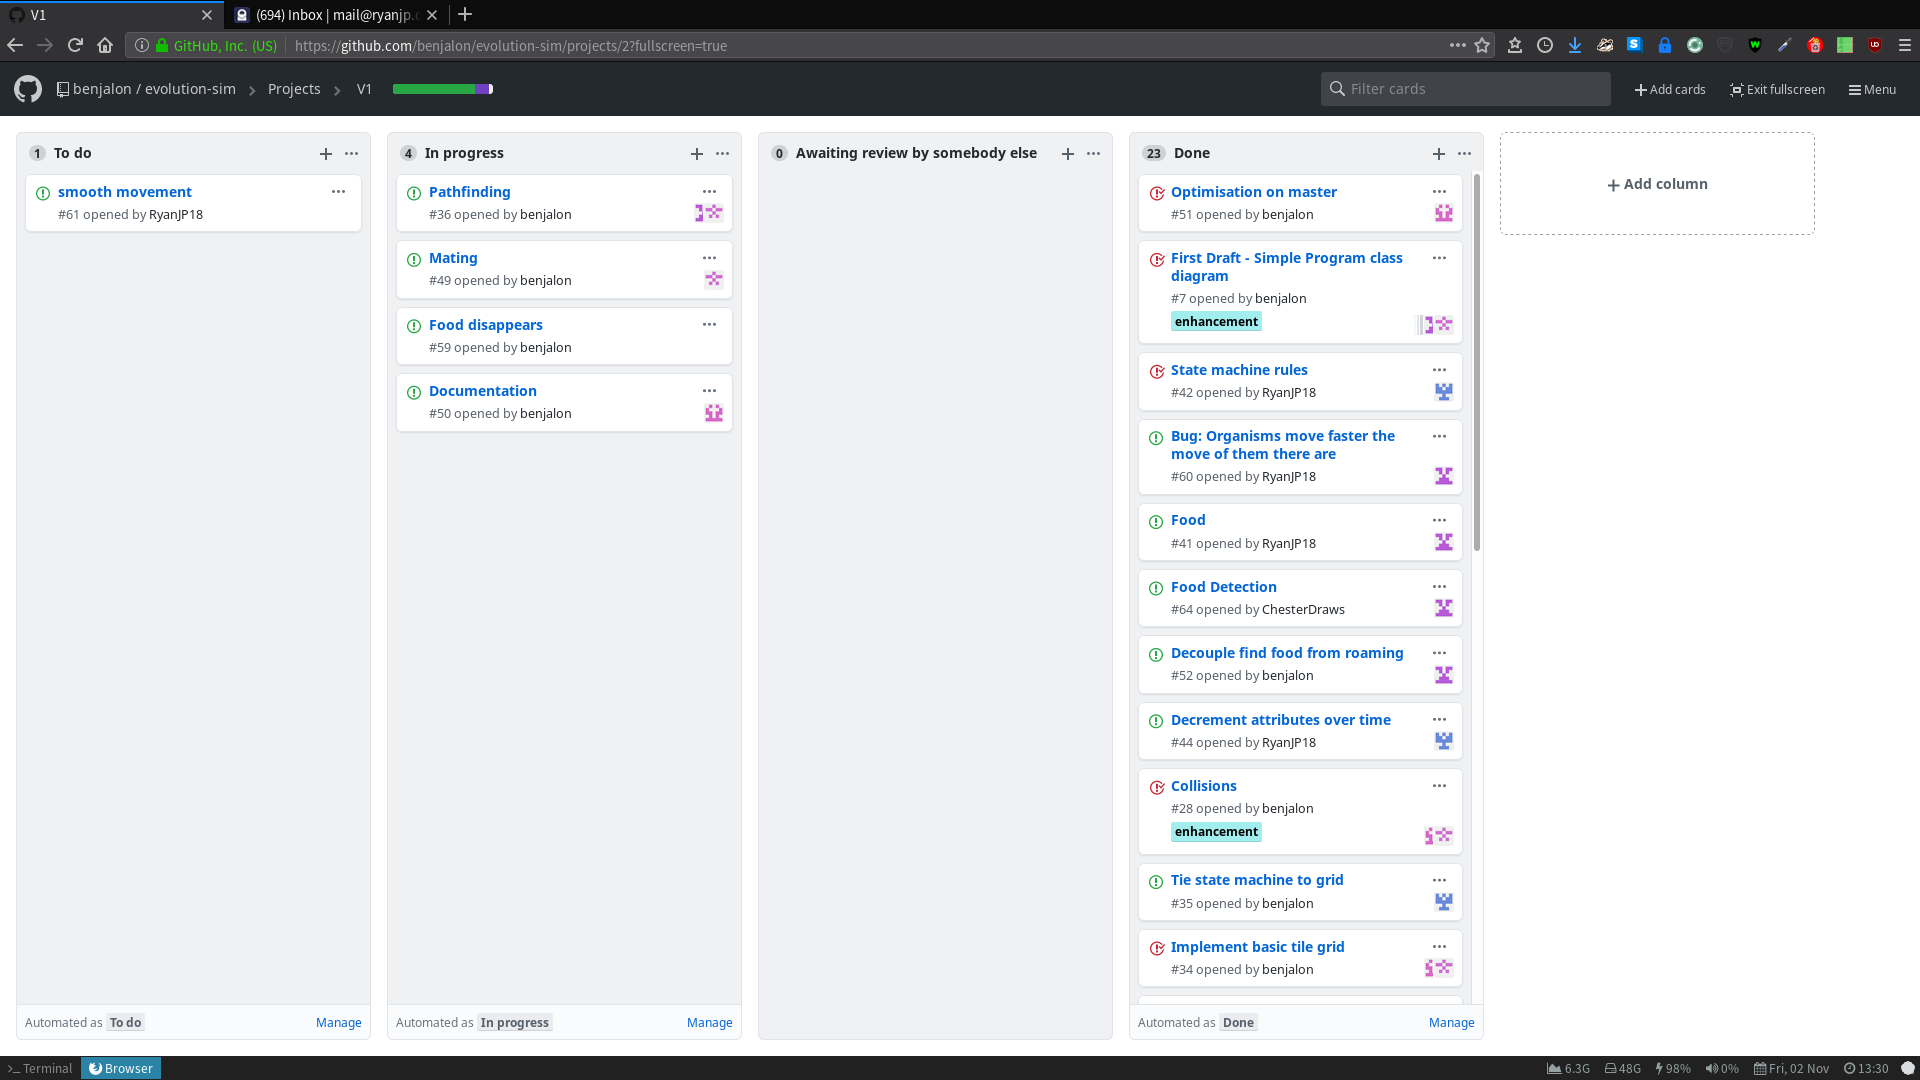
\includegraphics[width=0.8\textwidth]{gitproj}
	\caption{GitHub Project Board - Each of these boards represents one full sprint and one version of the software. When all of the issues are completed, the board is closed and a sprint planning meeting occurs.}\label{gitboard}
\end{figure}

\begin{figure}[H]
	\centering
	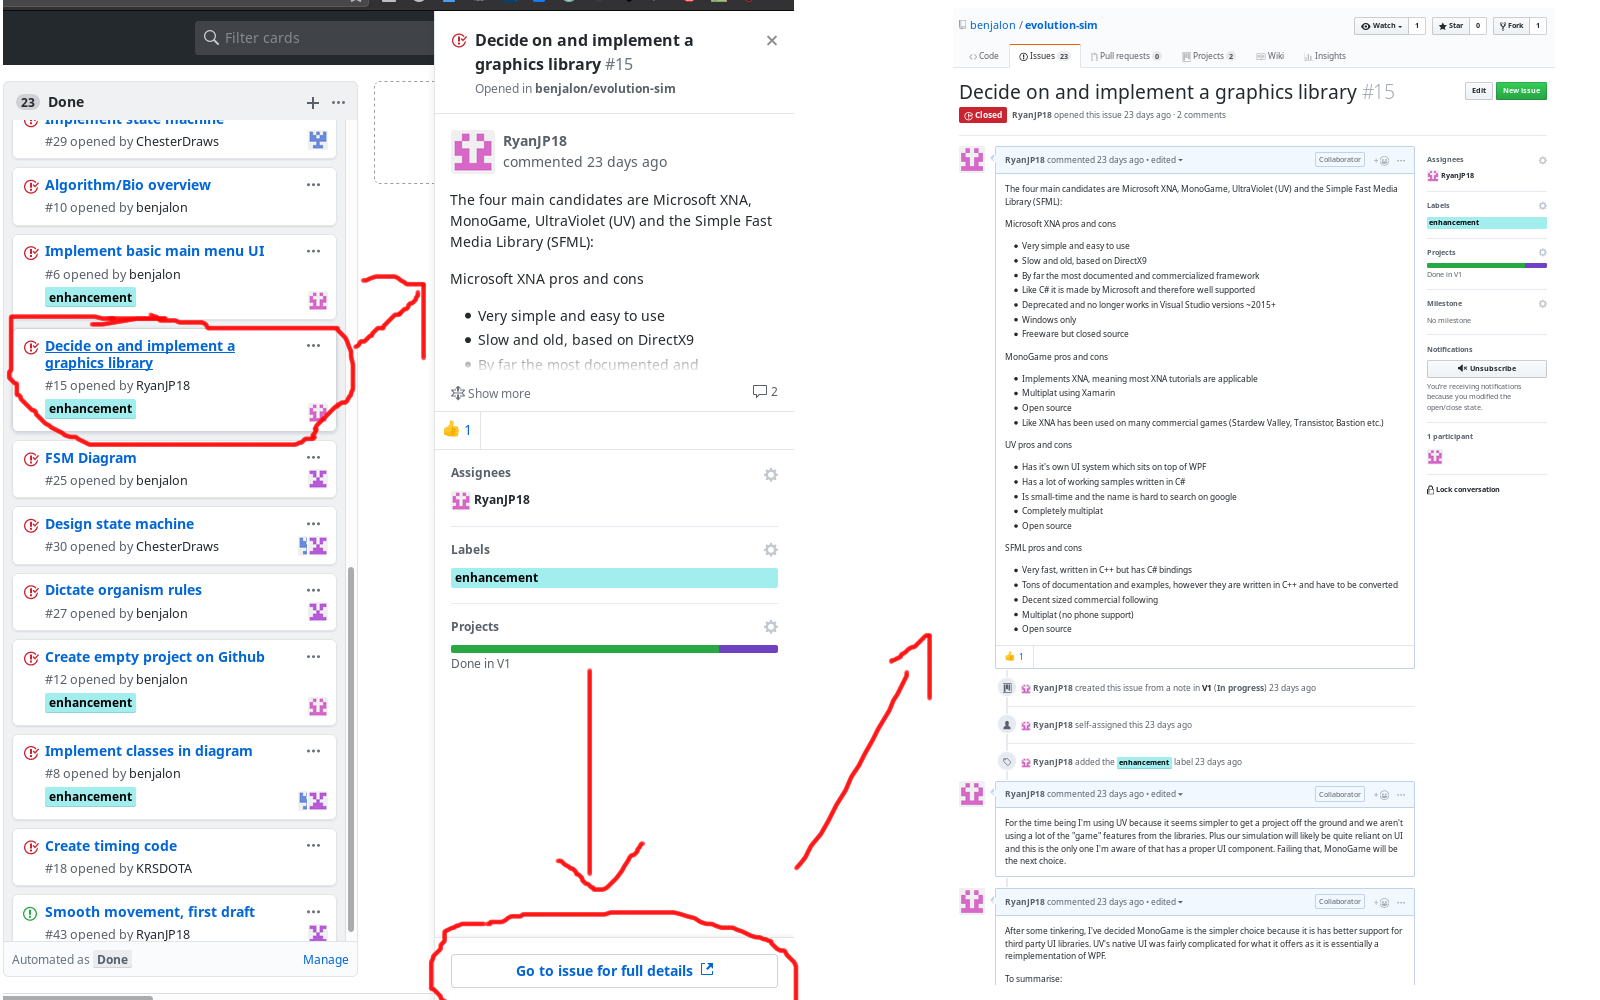
\includegraphics[width=0.8\textwidth]{gitissuetrack}
	\caption{GitHub Issue Tracking - Issues are created during sprint planning meetings, where necessary the person working on the task is expected to update the ticket with information that will need to be communicated to the team or included within any reports.}\label{gitissue}
\end{figure}

Within Git, each ticket is undertaken on its own branch and merged to master when completed. There is a lock on the master branch to prevent direct commits to enforce this rule, furthermore before a branch can be merged to master there is a further lock to ensure that a pull request is submitted and checked by at least one other person. This system helps ensure the quality of master for branching at all times, avoiding situations where development is halted due to a buggy code-base. Additionally, pull requests can function as a form of white-box testing as discussed in \ref{testing}.

Other project management tools include Microsoft OneNote for collaborative documentation and WhatsApp for quick discussion and scheduling.

\subsection{Versioning System}\label{versioning}
In keeping with the spirit of iterative development, the projects aim to produce a new product at the end of each sprint in order to keep systems well-rounded and stay on schedule. This also means that at any given time, the active project board matches the current release version. During sprint planning meetings, issues for the upcoming version are created against the MosCoW analysis \ref{moscow}:

\smallskip 
\begin{tabular}{c|p{0.7\textwidth}|l}
	Version & Goal & Deadline \\ \hline
	0 & A proof of concept to test the chosen technologies & Tuesday week 2 \\ \hline
	1 & A fully functioning basic simulation with all of the "Must Have" components from the MoSCoW analysis & Friday week 6 \\ \hline
	2 & Improvements on V1 simulation with tasks taken from the "should have" objectives. In particular, an advanced path finding algorithm such as A*, improved crossover algorithm, carnivores and a better time system. & Undecided \\ \hline
	3+ & Undecided & Undecided \
\end{tabular}
\smallskip 

\section{Code Architecture}\label{architecture}
The SOLID principles define five guidelines to ensure code is maintainable and easy to understand [\cite{kelmendi}]: 
\begin{itemize}
	\item Single Responsibility: Every class should have only one responsibility to prevent the class being susceptible to requirement changes.
	\item Open-Closed: Classes should be open to extension but abstraction should be used to avoid the need for rewrites on the extended code.
	\item Liskov Substitution: Derived and base classes should be substitutable.
	\item Interface Segregation: Keep interfaces simple to avoid bulk from implementing unnecessary properties.
	\item Dependency Inversion: Keep abstract code abstract by avoiding dependencies on low level code.
\end{itemize}

While these principles each affect the architecture in some way, in particular a great deal of effort is made to ensure that each class has a single responsibility. An example of this is in separating the Grid from the StateMachine despite the fact that they operate on similar areas of the simulation. The Grid is used as the "graphical brain", positioning organisms and drawing them at their positions, whereas the StateMachine is used as the "logical brain", dictating the behaviour which causes the organisms to be repositioned in the first place. Furthermore, the use of MapItem as a swappable base for Organism and Food would not work if the Liskov Substitution principle was not applied.

To ensure a clean and consistent code-base, the official Microsoft C\# conventions are applied where possible. Notable examples include placing braces on a new line, using camelCase for variable names and avoiding one line if statements [\cite{microsoft}].


\section{State Management}\label{statemanagement}
[TODO: Improve this]
Organism Behaviour – First Draft

1) Default organism state is “Roaming”.
a. From roaming, an organism can transition to “Seeking Food” or “Seeking Mate”.
2) If an organism is seeking food, it is simply roaming, with the added fact that if it is within a certain range of food, it will go towards it and consume it.
3) If an organism is seeking a mate, it is simply roaming, with the added fact that if it is within a certain range of a mate WHO IS ALSO SEEKING A MATE, it will go towards it and mate.
a. If whilst “Seeking Mate”, the organism becomes Hungry, it will transition to “Seeking Food”. End Goal: Biological Evolution Sandbox
b. What do we want?
i. End game, stable ecology
1. Net number of organisms don’t change
ii. Food, vegetation, other organisms
iii. Water
1. Some organisms can go in water
iv. Weatherdo not need to handle such specific details
1. Hot cold
2. Types of weather
v. Statistics
vi. A log
vii. Dis3ease
viii. Natural Disaster
ix. Terrain
x. Live Edit of organisms
c. Tile based graphicsOnce it has eaten sufficiently, it will go back to default state of roaming.

\section{Crossover Algorithm}\label{crossover}
The crossover algorithm is currently a work in progress.

\section{Grid System}\label{grid}
A common method of implementing movement in a simulation is through the use of a grid. This is a useful approach because by constricting organism movement to a set of definite positions, the number of movement states becomes finite and therefore better lends itself to algorithms such as pathfinding. In terms of efficiency, a grid also reduces the need for collision detection between simulation elements as when an organism wishes to move from one tile to another, the grid can simply accept or reject the move based on whether the destination tile is occupied. On the other hand, this limited movement is less realistic and does not necessarily reduce code complexity as the grid must constantly be made aware of the positions of its elements which requires a fair amount of manipulation to its arrays. 

In terms of the code, Grid refers to a management class which keeps track of the Tile positions in addition to some simple methods for interacting with them, for example to check whether a given Tile is occupied. In order to achieve this, the Grid contains a jagged two dimensional array of type Tile, where each index within it refers to a Tile's actual position on the screen.

[TODO: matrix/2d array image here]

When an organism wishes to move, a method on the Grid called MoveMapItem is passed the MapItem requesting to move with the destination it wishes to move to. Since Tiles are always in fixed positions from the simulation start, the Grid simply has to look up the destination from its fixed position array and check whether it is occupied and then ensure that the MapItem position is adjacent.

\section{Path Finding Algorithm}\label{pathfinding}
[TODO: DFS vs Dijkstra's vs A* algorithms, why pathfinding is necessary]

\section{Optimisation}\label{optim}
Optimisation is considered an area of importance due to the simulation's requirement in handling a large number of organisms without noticeable lag. By default, MonoGame's render loop calls two methods at a speed of sixty times per second: update and draw. Should the logic fail to complete within this ~16-17ms time-frame then it delays the draw call, which lowers the simulation's frame-rate. This has further knock-on effects where the draw calls become progressively more delayed and eventually cause input lag on the UI.

The update method is essentially the primary path through the code and handles all of the computation and organism logic. This method calls into several for loops to cycle through the various organisms and map items which make up the simulation. There can be several hundred objects to iterate through during any given Update loop, which as previously mentioned occurs sixty times per second. Keeping this entire iteration within the acceptable ~16-17ms time limit has requires consideration from an optimisation perspective.

Optimisation is a task better left until necessary following the argument that "premature optimization is the root of all evil [...]" \cite{knuth}, as doing so before it is necessary wastes time, introduces bugs and makes code less readable. However, at several points during the project, particularly during the first round of pathfinding implementation, performance was considered to be a problem. The A* pathfinding algorithm [\ref{pathfinding}] requires that the program keep track of open, closed and expanded nodes within various collections and though there are many ways to implement the algorithm, they often involve some degree of manipulation. As previously mentioned, the update method is already within the sixty per second game loop and then within another nested loop for each of the tiles [\ref{grid}]. Before delving into loop micro-optimisation, the amount of loops and collection manipulation was cut down as much as possible.

To improve the performance of these loops, the standard loop micro-optimisations are applied. Variables are declared outside of the loop scope, collection length is cached locally ahead of time and high precision calculations are avoided. For example, the DateTime object was initially used to time organism movements but because it uses double precision values, calculations were causing a large slowdown so it was swapped for the better optimised GameTime object. Finally, the grid stores its tiles within a two dimensional array which could potentially be implemented in C\# in two different ways: multi-dimensional arrays and jagged arrays. A jagged array is an array of arrays and allows these inner arrays to vary in length, whereas a multi-dimensional is a natural 2D array where the column count is uniform. The grid stores its tiles in a jagged array because within a jagged array, even if the arrays are the same length, it is able to iterate faster than a multi-dimensional array.

Finally, though it caused issue in this instance, from an architecture perspective the grid system is also a form of optimisation. By constricting organism movements to a grid the simulation is able to cut down on the need for collision detection by having organisms request their moves to the grid, which then makes the decision of whether the move is legal. Collision detection would otherwise have been a bottleneck for the system which would have been exponentially slower as more organisms are added because each organism would need to check the position all of the others. With the tile system in place however, there are always a set number of tiles to iterate over rather than a growing list of organisms with references to each of the others.

\section{Multi-threading}
To better improve the performance of the pathfinding, it is currently being moved to different threads. This is a work in progress.

\chapter{Implementation} \label{implementation}

\section{Tools}\label{tools}
Three programming languages were considered for the project: C++, C\# and Java. The simulation was identified to have a large dependency on computation due to the fact that there could be upwards of one hundred organisms on screen at any one time and each of them would require state management, path finding and collision detection. For this reason, C++ seemed to be the natural choice due to the speed benefit of dynamic memory management. However, upon further research it was found that C\# had a more diverse set of 2D graphics libraries as C++ libraries were typically focused on 3D rendering. Finally, Java was considered because the bulk of the team's experience was with the language, though because C\# can be used as a drop-in replacement for Java this was seen as another benefit in using C\#.

Since the availability of tools is dependant on the chosen language, the decision of a graphics framework was next. A comparison was made between several popular 2D graphics libraries, the four main candidates being Microsoft XNA, MonoGame, UltraViolet (UV) and the Simple Fast Media Library (SFML):

\begin{center}
	\begin{tabular}{c|p{0.4\textwidth}|p{0.4\textwidth}}
		Library & Pros & Cons \\ \hline
		Microsoft XNA & \begin{itemize}
			\itemsep0em
			\item Simple and easy to use
			\item Very well documented
			\item Well-used commercially
			\item Supported by Microsoft who also made C\#
		\end{itemize} & \begin{itemize}
			\itemsep0em
			\item Slow and old, based on DirectX9
			\item Deprecated and no longer works in Visual Studio 2015+
			\item Windows only
			\item Closed source
		\end{itemize} \\ \hline
		MonoGame & \begin{itemize}
			\itemsep0em
			\item Based on XNA with the same syntax, all of the XNA documentation is applicable
			\item Multi-platform but requires Xamarin
			\item Open source
			\item Has seen use on commercial games (Stardew Valley, Transistor, Bastion etc.)
		\end{itemize} & \begin{itemize}
			\itemsep0em
			\item Convoluted asset management system
		\end{itemize} \\ \hline
		UV & \begin{itemize}
			\itemsep0em
			\item Has a built in UI framework based on Windows Presentation Foundation (WPF)
			\item Truly multi-platform
			\item Open source
		\end{itemize} & \begin{itemize}
			\itemsep0em
			\item Convoluted asset management system
			\item Limited documentation, small time
			\item Little to no commercial use
		\end{itemize} \\ \hline
		SFML & \begin{itemize}
			\itemsep0em
			\item Very fast, written in C++ but has C\# bindings
			\item Well documented
			\item Some commercial use
			\item Multi-platform but no phone support
			\item Open source
		\end{itemize} & \begin{itemize}
			\itemsep0em
			\item C\# bindings are slightly behind on updates
			\item Examples and documentation are written in C++ and require converting
			\item Syntax is not as simple as other frameworks
		\end{itemize} \\
	\end{tabular}
\end{center}

Though UV was initially chosen due to its built-in UI support, where UI was deemed a core component of the simulation, the lack of documentation and convoluted XML system for managing assets meant that MonoGame was chosen instead. A third party UI library, GeonBit.UI, was chosen because although any 2D graphics framework is capable of rendering UI using sprite assets, one of the project requirements [\ref{requirements}] was that the UI have a professional look. Additionally, UI elements such as lists and radio buttons were considered a likely requirement and would be difficult to implement with a graphics approach.

\section{Proof of Concept}
A proof of concept was made with the chosen technologies before any further planning took place because the team wanted to avoid a situation where the UML modelling and code architecture was planned according to a language or tool that was then realised to be a poor fit for the project. The aim of the proof of concept was to simply draw a number of organisms to the screen using the chosen graphics framework which could be manipulated using a simple place-holder UI.

\begin{figure}[H]
	\caption{Proof of Concept}\label{poc}
	\centering
	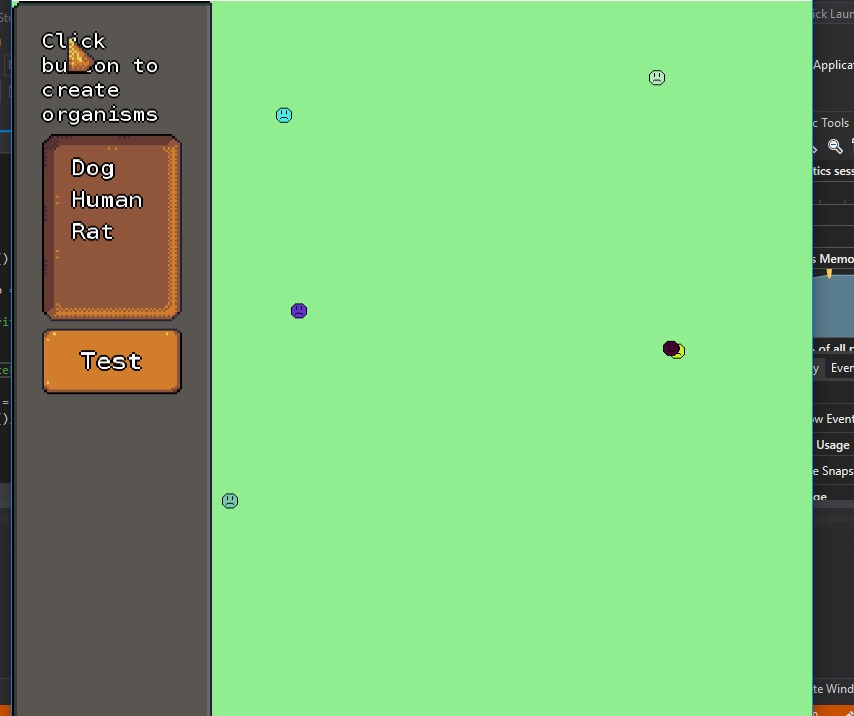
\includegraphics[width=0.8\textwidth]{poc}
\end{figure}

The proof of concept was deemed a success as it was able to create organisms using the UI button, move them around and render them without lag.
\section{Modelling}
The class diagram Figure~\ref{classdiagram} was continually updated throughout the project and although it saw many changes, certain key themes remained constant throughout.

An important architectural decision made from the outset was to ensure the separation of concerns between the graphics, simulation and UI. It was decided that the graphical component should provide a representation of the simulation's output, but that they should be kept unaware of the inner workings of the other to better decouple their behaviour. Likewise, while the UI would be able to interact with the simulation, there was no need to have this behaviour tied in any way to the intricacies of it. As such, the relationship between the three key areas can be observed as limited on the class diagram.

Another theme present in the class diagram is abstraction. Through inheritance, MapItems are kept as generic inhabitants by the Tiles of the Grid. This means that the Grid can manage its Tiles and their inhabitant MapItems without particular knowledge of whether they are Organisms, Food or Obstacles, simplifying the implementation.

\section{Version 1}
[TODO: Write this, include the end of sprint meeting (performance issues)]

\section{Version 2}
Version 2 is currently a work in progress.

\chapter{Testing}\label{testing}

This section will be about the following:
\begin{itemize}
	\itemsep0em
	\item Pull requests as a form of white-box testing during development
	\item Unit testing with the built in C\# tools
	\item Experimenting with several untouched simulations to ensure equilibrium is reached 
	\item Experimenting with editing attributes and reaching equilibrium, likewise with natural disasters and disease
	\item A section on the bug fixing ticket system in place \label{bugfixing}
\end{itemize} 

\chapter{Discussion}\label{discussion}

This section will be about the following:
\begin{itemize}
	\itemsep0em
	\item Discussion of testing and experiment results
	\item Issues encountered: frequent rewrites, tangled state management early on, slowdown and lag, inconsistent coding standards, pathfinding necessitating optimisation and multiple threads, pull request system 
	\item What went well/badly
	\item What could be improved
\end{itemize} 

\chapter{Conclusion and Future Work}\label{conclusion}

This section will conclude the MoSCoW analysis, discuss shortcomings and future developments with more time. It will avoid subjective opinions, rants and excuses.

\bibliographystyle{unsrt}
\bibliography{references}

\chapter*{Contributions}

The team has agreed on a 25\% contibution each as of the time of writing. Note that these contributions are to date and not representative of planned features. 
\smallskip 
\begin{center}
	\begin{tabular}{c|p{0.4\textwidth}|p{0.4\textwidth}}
		Member & Ownership of/Major Contributions & Assisted on/Minor Contributions \\ \hline
		Benjamin Longhurst & \begin{itemize}
			\itemsep0em
			\item Project management [\ref{projectmanagement}]
			\item A* Pathfinding [\ref{pathfinding}]
		\end{itemize} & \begin{itemize}
			\itemsep0em
			\item Grid/tile system [\ref{grid}]
			\item Bio. algorithms research [\ref{crossover}]
		\end{itemize} \\ \hline
		Rupert Hammond & \begin{itemize}
			\itemsep0em
			\item State management [\ref{statemanagement}]
			\item State machine rules
			\item Bio. algorithms research [\ref{crossover}]
			\item Organism attributes
		\end{itemize} & \begin{itemize}
			\itemsep0em
			\item Bug fixing [\ref{bugfixing}]
			\item A* Pathfinding [\ref{pathfinding}]
		\end{itemize} \\ \hline
		Ryan Phelan & \begin{itemize}
			\itemsep0em
			\item Graphics/UI research and implementation [\ref{tools}]
			\item Grid/tile system [\ref{grid}]
			\item Optimisation [\ref{optim}]
			\item Report writing
		\end{itemize} & \begin{itemize}
			\itemsep0em
			\item Project management [\ref{projectmanagement}]
			\item Code architecture [\ref{architecture}]
		\end{itemize} \\ \hline
		Travis Payne & \begin{itemize}
			\itemsep0em
			\item Food system
			\item Movement logic
			\item Simulation flow [\ref{statemanagement}]
		\end{itemize} & \begin{itemize}
			\itemsep0em
			\item Code architecture [\ref{architecture}]
			\item Bug fixing [\ref{bugfixing}]
			\item A* Pathfinding [\ref{pathfinding}]
			\item Organism attributes
		\end{itemize} \\
	\end{tabular}
\end{center}
\smallskip
Other work such as the Proof of Concept, UML and analysis' were completed as a team with all members present.
\chapter*{Appendix A}

\begin{figure}[H]
	\caption{UML Class Diagram}\label{classdiagram}
	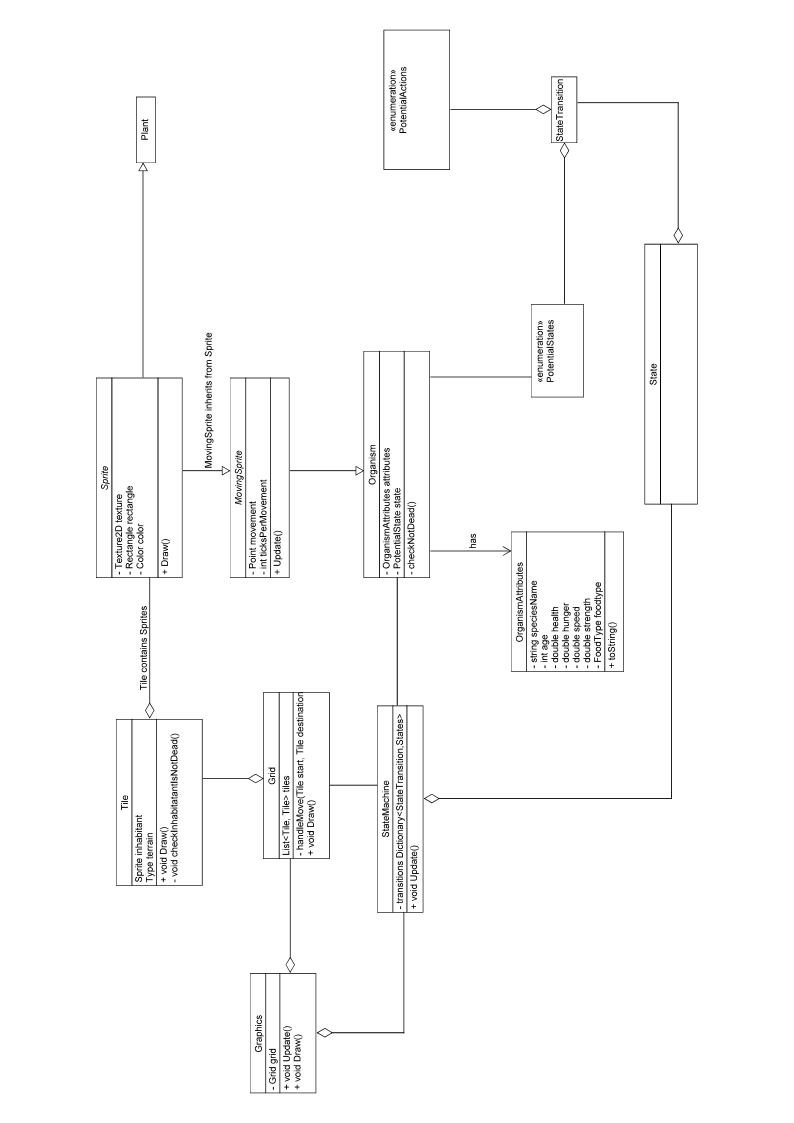
\includegraphics[width=\textwidth,height=\textheight]{class-diagram}
\end{figure}

\end{document}

